\documentclass[11pt,a4paper]{article}
\usepackage[utf8]{inputenc}
\usepackage[T1]{fontenc}
\usepackage[brazil]{babel}
\usepackage[a4paper,margin=2.3cm]{geometry}
\usepackage{graphicx}
\usepackage{booktabs}
\usepackage{amsmath}
\usepackage{amssymb}
\usepackage{siunitx}
\usepackage{xcolor}
\usepackage{caption}
\usepackage[colorlinks=true,linkcolor=blue,urlcolor=blue]{hyperref}

\graphicspath{{../resultados/}}
\captionsetup{font=small,labelfont=bf}
\setlength{\parskip}{0.4em}
\setlength{\parindent}{0pt}

\title{\textbf{Laboratório 03 --- Granulometria Morfológica}\\[0.3em]
\large Caracterização de texturas da base KTH-TIPS por assinaturas granulométricas}
\author{Saymon Coppi de Oliveira Silva\\ \small Visão Computacional --- PPG em Ciência da Computação, ICT/UNIFESP}
\date{\today}

\begin{document}
\maketitle

\begin{abstract}
\noindent Este trabalho investiga o uso de \textbf{granulometria morfológica} para
caracterizar texturas em diferentes escalas. Cada imagem é representada por uma
\emph{assinatura granulométrica} (pattern spectrum) obtida por aberturas
morfológicas em tons de cinza com elementos estruturantes de tamanho crescente.
Usando três classes da base KTH-TIPS (\texttt{corduroy}, \texttt{cotton} e
\texttt{linen}), mostramos que a assinatura captura a escala característica de
cada material: os tecidos finos (\texttt{cotton}, \texttt{linen}) concentram sua
massa em escalas pequenas ($r\!\approx\!2$) e possuem assinaturas quase
sobrepostas, enquanto o veludo cotelê (\texttt{corduroy}) exibe um pico
secundário em escala grande ($r\!\approx\!10$), correspondente às suas ranhuras.
Um classificador 1-NN \emph{leave-one-out} sobre as assinaturas atinge
\textbf{93{,}3\%} de acurácia, confirmando que o descritor é útil para
distinguir os materiais e que a maior confusão ocorre justamente entre os dois
tecidos finos.
\end{abstract}

% ---------------------------------------------------------------------------
\section{Base utilizada e classes selecionadas}

Foi utilizada a base \textbf{KTH-TIPS} (\emph{Textures under varying Illumination,
Pose and Scale}), na versão em tons de cinza $200\times200$
(\url{https://www.csc.kth.se/cvap/databases/kth-tips/download.html}). Cada
material possui 81 imagens, capturadas em 9 escalas $\times$ 3 poses $\times$ 3
condições de iluminação.

Selecionamos \textbf{3 classes} e \textbf{20 imagens por classe} (60 imagens no
total), dentro da faixa recomendada (10--20 por classe). As classes foram
escolhidas para produzir um cenário informativo de comparação --- \emph{dois
materiais semelhantes e um distinto}:

\begin{itemize}
  \item \texttt{corduroy} (veludo cotelê): tecido com \textbf{ranhuras verticais
        regulares e grossas} --- estrutura de escala grande.
  \item \texttt{cotton} (algodão): tecido de \textbf{trama fina} e regular.
  \item \texttt{linen} (linho): tecido de \textbf{trama fina}, visualmente
        próximo do algodão.
\end{itemize}

Todas as imagens são mantidas em tons de cinza e já possuem tamanho uniforme
($200\times200$); o código ainda garante o redimensionamento por interpolação de
área quando necessário.

\begin{figure}[h]
  \centering
  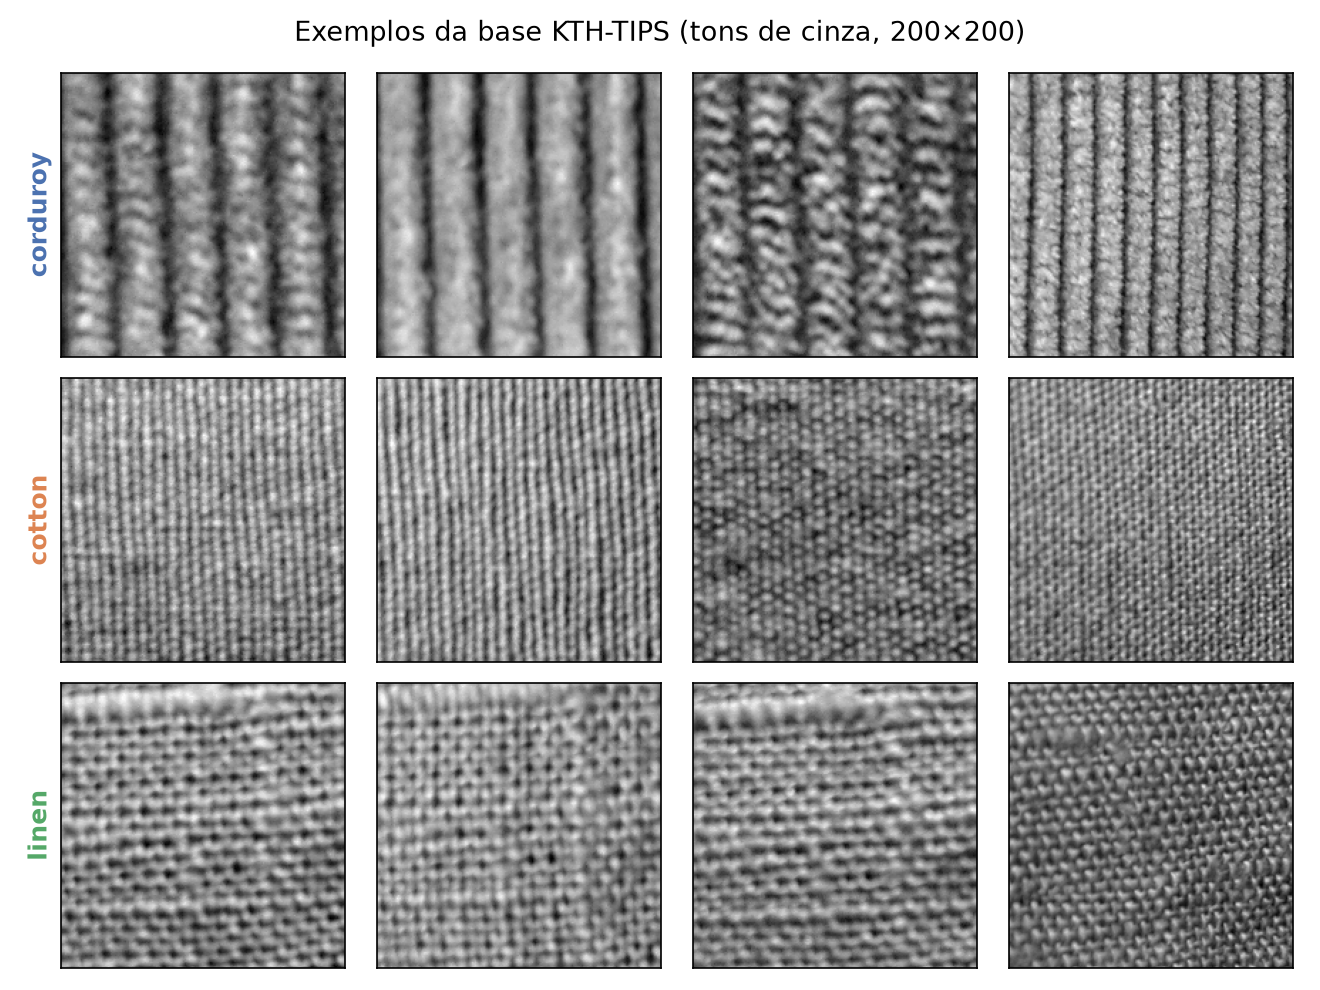
\includegraphics[width=0.85\textwidth]{exemplos_base.png}
  \caption{Exemplos das três classes. As ranhuras largas do \texttt{corduroy}
  (linha superior) contrastam com as tramas finas de \texttt{cotton} e
  \texttt{linen}, que são difíceis de distinguir a olho nu.}
\end{figure}

% ---------------------------------------------------------------------------
\section{Abordagem: assinatura granulométrica}

A granulometria morfológica descreve a distribuição de tamanhos das estruturas
de uma imagem através de \textbf{aberturas} sucessivas por elementos
estruturantes cada vez maiores~\cite{maragos1989}. Seja $f$ a imagem em tons de
cinza e $rB$ o elemento estruturante $B$ escalado por $r$. A abertura
$\gamma_{rB}(f)$ é anti-extensiva: quanto maior $r$, mais estruturas finas são
removidas. Definimos o ``volume'' de intensidade
\begin{equation}
  V(r) = \sum_{x} \gamma_{rB}(f)(x), \qquad V(0)=\sum_x f(x).
\end{equation}
Como $V(r)$ é monotonicamente decrescente, a \textbf{curva granulométrica
cumulativa} (distribuição de tamanhos) é
\begin{equation}
  \Phi(r) = 1 - \frac{V(r)}{V(0)}, \qquad \Phi(r)\in[0,1],
\end{equation}
e a \textbf{assinatura granulométrica} (\emph{pattern spectrum}) é a sua
derivada discreta, normalizada:
\begin{equation}
  \mathrm{PS}(r) = \frac{V(r-1) - V(r)}{V(0)} \;\ge\; 0.
\end{equation}
$\mathrm{PS}(r)$ mede a fração da ``massa'' da imagem composta por estruturas de
tamanho exatamente $r$; é, portanto, um histograma de escalas que independe do
brilho global (graças à normalização por $V(0)$).

\paragraph{Implementação.} O código é escrito em \textbf{Python} usando
\texttt{OpenCV} (aberturas em tons de cinza via \texttt{cv2.morphologyEx} com
\texttt{MORPH\_OPEN}), \texttt{NumPy}, \texttt{Matplotlib} e \texttt{pandas}.
Empregamos elemento estruturante \textbf{isotrópico em forma de disco}
(\texttt{MORPH\_ELLIPSE}) de raio $r$ (tamanho $2r+1$), varrendo a faixa de
escalas $r = 1,2,\dots,25$. A escolha de um disco (em vez de um quadrado) evita
favorecer direções específicas, o que é adequado para texturas de orientação
arbitrária. O núcleo do método resume-se a:

\begin{quote}\small\ttfamily
for r in 1..R:\\
\hphantom{xx}aberta = morphologyEx(f, MORPH\_OPEN, disco(r))\\
\hphantom{xx}V[r] = soma(aberta)\\
PS[r] = (V[r-1] - V[r]) / V[0]
\end{quote}

% ---------------------------------------------------------------------------
\section{Assinaturas individuais e médias por classe}

A Figura~\ref{fig:individuais} mostra, para cada classe, as 20 assinaturas
individuais (linhas finas) e a assinatura \textbf{média} (linha tracejada). A
Figura~\ref{fig:comparacao} sobrepõe as três médias com uma banda de $\pm 1$
desvio-padrão.

\begin{figure}[h]
  \centering
  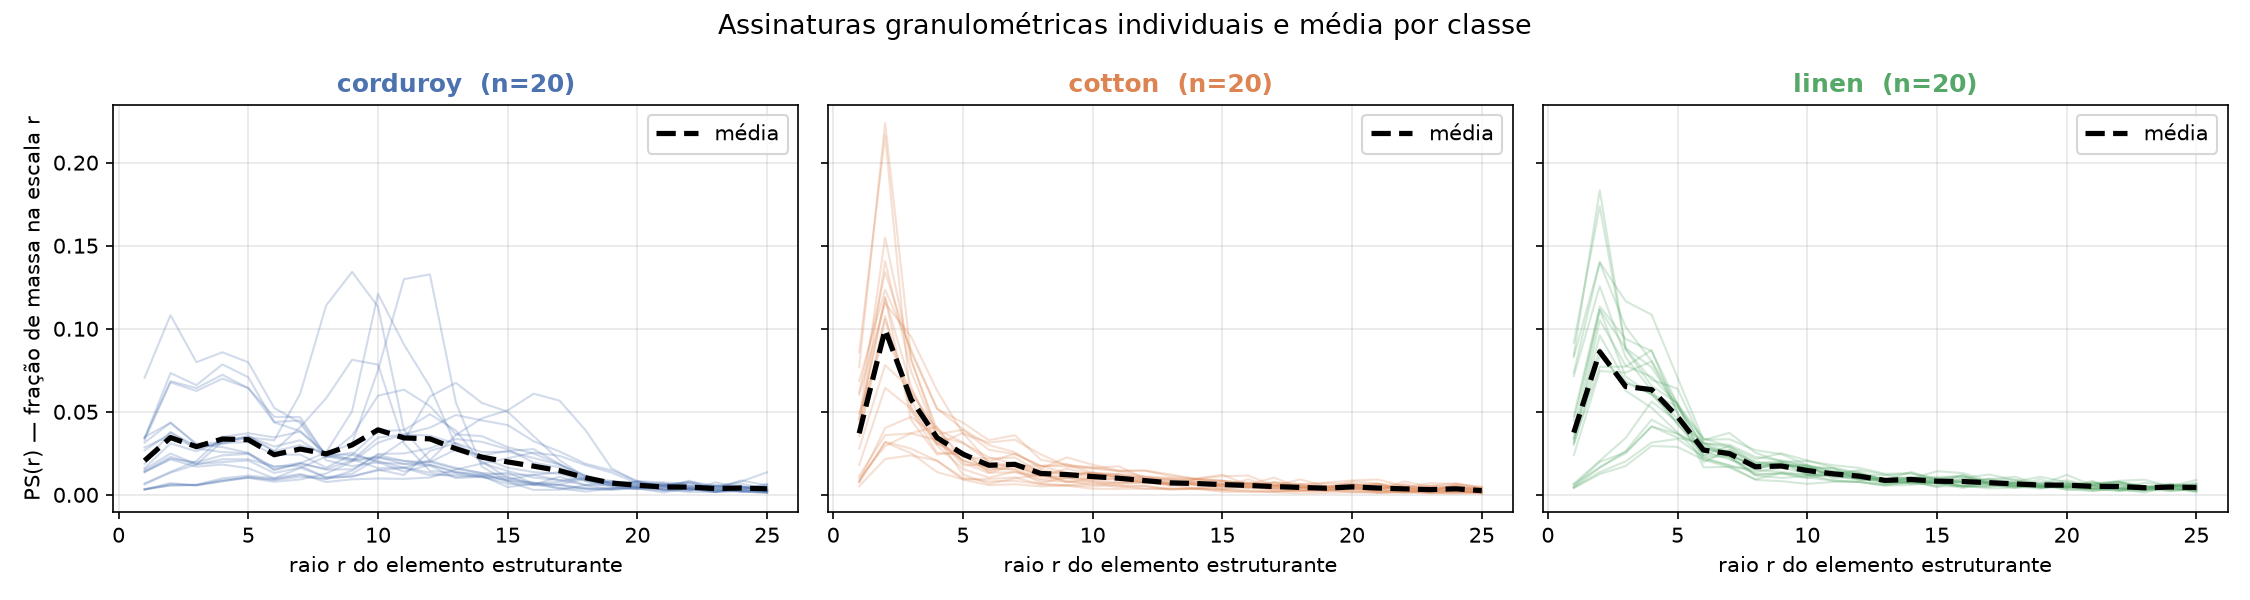
\includegraphics[width=\textwidth]{assinaturas_individuais.png}
  \caption{Assinaturas granulométricas individuais (finas) e média (tracejada)
  por classe. \texttt{cotton} e \texttt{linen} têm pico acentuado em
  $r\!\approx\!2$; \texttt{corduroy} espalha massa por escalas maiores, com
  realce em torno de $r\!\approx\!10$.}
  \label{fig:individuais}
\end{figure}

\begin{figure}[h]
  \centering
  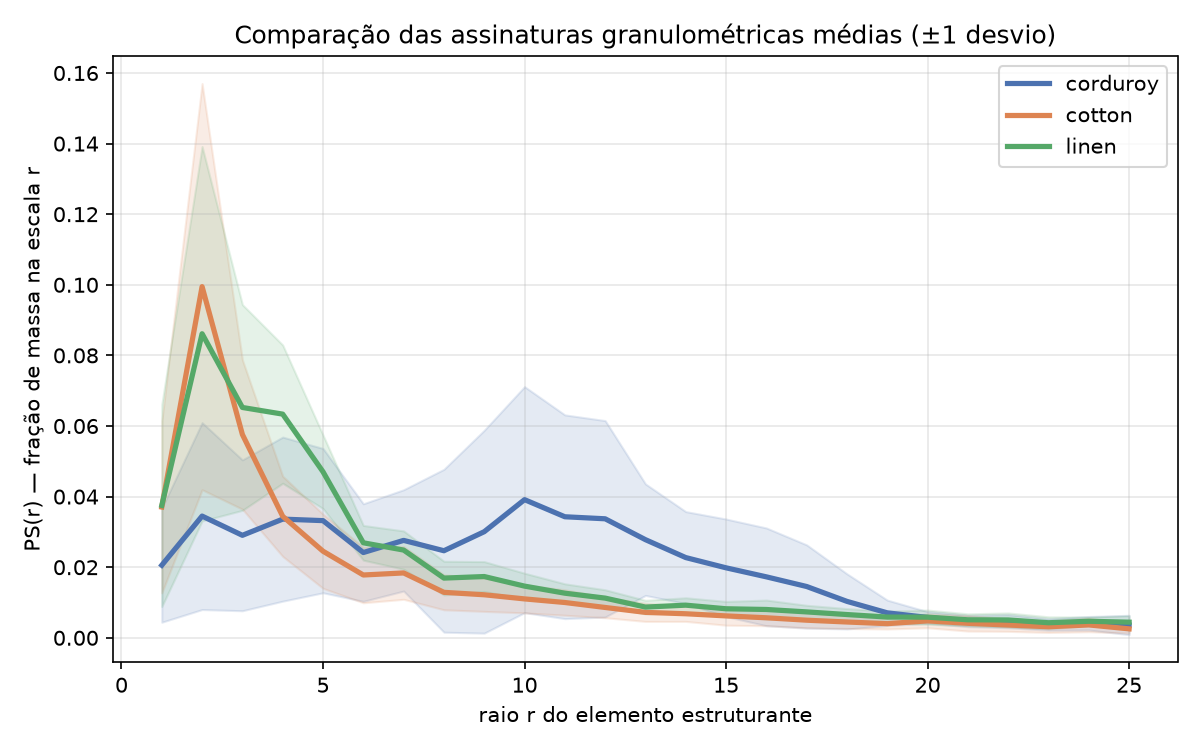
\includegraphics[width=0.78\textwidth]{assinaturas_comparacao.png}
  \caption{Comparação das assinaturas médias ($\pm 1$ desvio). O pico secundário
  do \texttt{corduroy} em $r\!\approx\!10$ é a assinatura das suas ranhuras.}
  \label{fig:comparacao}
\end{figure}

A Tabela~\ref{tab:resumo} resume o raio de pico e a massa total de cada
assinatura média. A curva cumulativa $\Phi(r)$ (Figura~\ref{fig:cumulativa})
mostra a mesma informação de forma integrada: \texttt{cotton} e \texttt{linen}
saturam rapidamente (estruturas pequenas), enquanto \texttt{corduroy} cresce de
modo mais gradual, só se estabilizando após capturar suas ranhuras.

\begin{table}[h]
  \centering
  \small
  \caption{Resumo das assinaturas médias por classe.}
  \label{tab:resumo}
  \begin{tabular}{lcc}
    \toprule
    Classe & Raio de pico $r^\ast$ & Massa total $\sum_r \mathrm{PS}(r)$ \\
    \midrule
    \texttt{corduroy} & 10 & 0{,}511 \\
    \texttt{cotton}   & \phantom{0}2 & 0{,}405 \\
    \texttt{linen}    & \phantom{0}2 & 0{,}507 \\
    \bottomrule
  \end{tabular}
\end{table}

\begin{figure}[h]
  \centering
  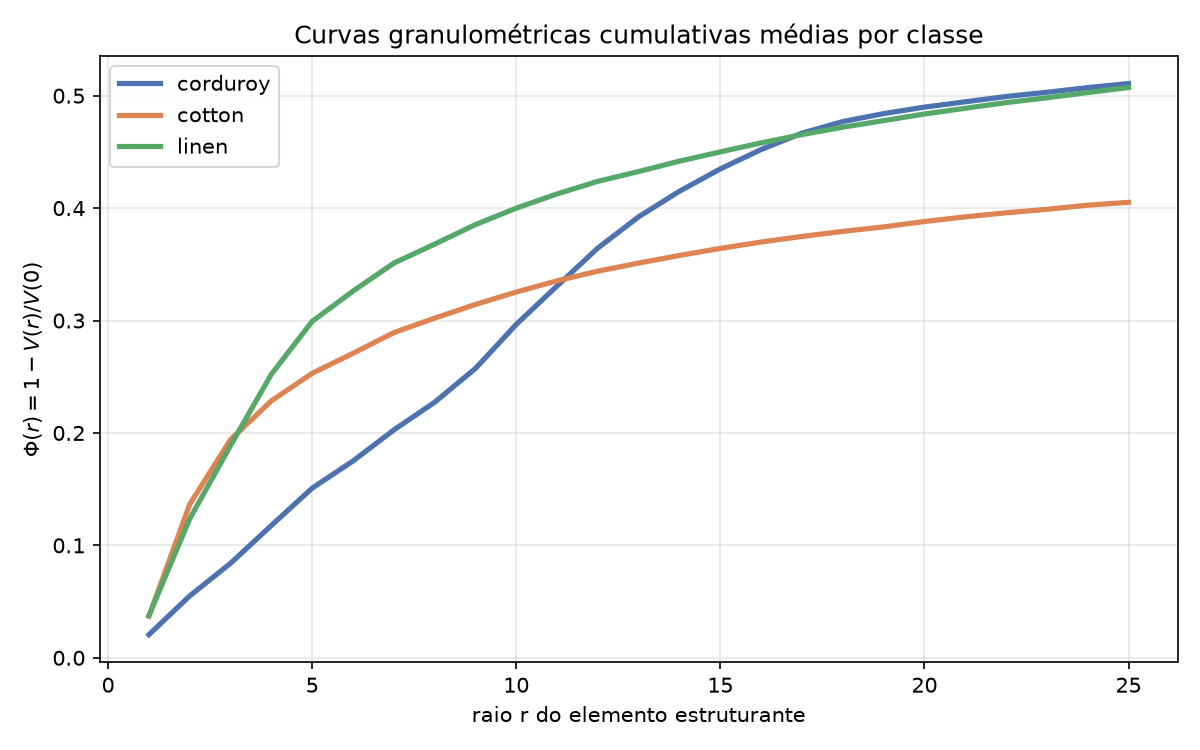
\includegraphics[width=0.72\textwidth]{curvas_cumulativas.png}
  \caption{Curvas granulométricas cumulativas médias $\Phi(r)$.}
  \label{fig:cumulativa}
\end{figure}

% ---------------------------------------------------------------------------
\section{Comparação entre classes: semelhança e separabilidade}

\paragraph{Distância entre assinaturas médias.} A Tabela~\ref{tab:dist} apresenta
a distância $L_1$ entre as assinaturas médias. O par
\texttt{cotton}--\texttt{linen} é, de longe, o mais próximo ($0{,}129$),
enquanto \texttt{corduroy} está distante de ambos ($0{,}31$--$0{,}33$). Ou seja,
as \textbf{curvas mais semelhantes são as de \texttt{cotton} e \texttt{linen}}, e
a classe \textbf{mais fácil de separar é \texttt{corduroy}}.

\begin{table}[h]
  \centering
  \small
  \caption{Distância $L_1$ entre as assinaturas granulométricas médias.}
  \label{tab:dist}
  \begin{tabular}{lccc}
    \toprule
     & \texttt{corduroy} & \texttt{cotton} & \texttt{linen} \\
    \midrule
    \texttt{corduroy} & 0{,}000 & 0{,}327 & 0{,}311 \\
    \texttt{cotton}   & 0{,}327 & 0{,}000 & \textbf{0{,}129} \\
    \texttt{linen}    & 0{,}311 & \textbf{0{,}129} & 0{,}000 \\
    \bottomrule
  \end{tabular}
\end{table}

\paragraph{Separabilidade objetiva (1-NN \emph{leave-one-out}).} Para medir a
utilidade do descritor de forma quantitativa, classificamos cada imagem pelo
vizinho mais próximo (distância $L_1$ entre assinaturas), deixando-a de fora do
conjunto de referência. A acurácia é \textbf{93{,}3\%} (56 de 60). A matriz de
confusão (Figura~\ref{fig:confusao}) mostra que \textbf{todos os erros envolvem o
par \texttt{cotton}--\texttt{linen}} ou levam o \texttt{corduroy} a ser
confundido apenas quando sua imagem foi capturada em uma escala atípica --- nunca
há confusão sistemática com o veludo. Isso confirma numericamente a leitura
visual das curvas.

\begin{figure}[h]
  \centering
  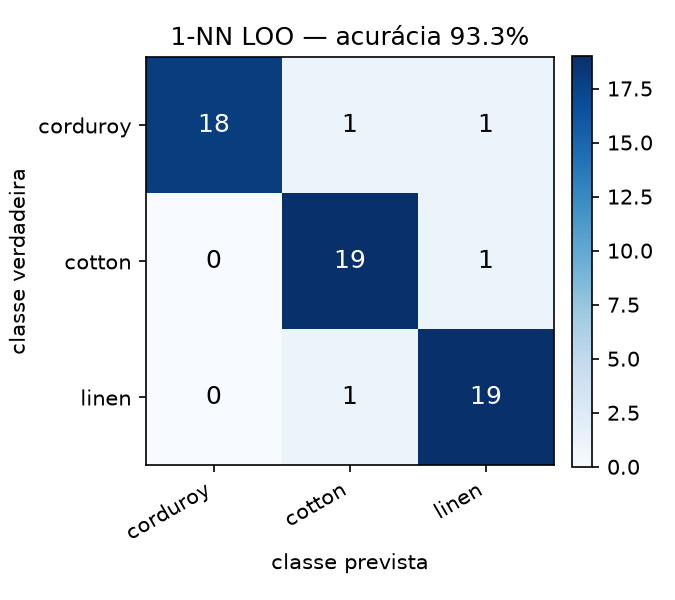
\includegraphics[width=0.5\textwidth]{matriz_confusao.png}
  \caption{Matriz de confusão do classificador 1-NN \emph{leave-one-out} sobre as
  assinaturas granulométricas.}
  \label{fig:confusao}
\end{figure}

% ---------------------------------------------------------------------------
\section{Efeito da faixa de escalas}

A faixa de raios escolhida é \textbf{determinante} para o poder discriminativo da
assinatura. Observações:

\begin{itemize}
  \item \textbf{Faixa curta demais.} Limitar a $r \le 5$ capturaria bem os
        tecidos finos (pico em $r\!=\!2$), mas \textbf{perderia o traço mais
        distintivo do \texttt{corduroy}}, cujo pico está em $r\!\approx\!10$. As
        três classes pareceriam então mais semelhantes do que realmente são.
  \item \textbf{Faixa longa demais.} Para $r \gtrsim 18$ as três curvas já
        decaíram a valores próximos de zero (ver Figuras~\ref{fig:individuais}
        e~\ref{fig:comparacao}); raios adicionais quase não carregam informação e
        apenas encarecem o cálculo (a abertura fica mais custosa com $r$).
  \item \textbf{Escolha adotada.} A faixa $r\in[1,25]$ cobre com folga o pico do
        \texttt{corduroy} e a cauda de todas as classes, sendo um bom
        compromisso entre cobertura e custo. O valor $r_{\max}=25$ ($\approx 1/8$
        do lado da imagem) é uma regra prática razoável.
\end{itemize}

Vale notar que, como a KTH-TIPS mistura escalas de captura, uma mesma textura
aparece com granulometrias ligeiramente deslocadas --- efeito visível na
dispersão das linhas finas do \texttt{corduroy} na Figura~\ref{fig:individuais}.
Isso reforça a importância de uma faixa ampla o suficiente para acomodar essa
variação.

% ---------------------------------------------------------------------------
\section{Dificuldades encontradas}

\begin{itemize}
  \item \textbf{Definição da assinatura.} Havia mais de uma convenção possível
        (curva cumulativa $\Phi$ vs.\ pattern spectrum $\mathrm{PS}$). Adotamos o
        \emph{pattern spectrum} normalizado por ser um histograma de escalas mais
        interpretável, mantendo também a curva cumulativa para referência.
  \item \textbf{Normalização.} Sem dividir por $V(0)$, imagens mais claras
        produziriam assinaturas de maior amplitude, contaminando a comparação
        entre classes. A normalização por volume inicial resolveu isso.
  \item \textbf{Faixa de escalas.} Escolher $r_{\max}$ exigiu inspecionar as
        curvas: valores baixos escondiam o pico do \texttt{corduroy} e valores
        altos só acrescentavam ruído/custo.
  \item \textbf{Variação de escala da base.} A mistura de escalas de captura da
        KTH-TIPS aumenta a variância intraclasse do \texttt{corduroy} e explica
        os poucos erros de classificação dessa classe.
  \item \textbf{Custo computacional.} A abertura em tons de cinza com discos
        grandes é a etapa mais cara; redimensionar para $200\times200$ e usar
        \texttt{OpenCV} mantiveram o tempo total na casa de segundos.
\end{itemize}

% ---------------------------------------------------------------------------
\section{Conclusão}

A granulometria morfológica mostrou-se um descritor \textbf{útil e
interpretável} para caracterizar texturas em diferentes escalas. A assinatura
captura diretamente a escala das estruturas de cada material: pequenos raios para
tramas finas (\texttt{cotton}, \texttt{linen}) e um pico em escala grande para as
ranhuras do \texttt{corduroy}. A análise quantitativa confirma a leitura visual
--- as classes mais semelhantes são \texttt{cotton} e \texttt{linen}
(distância $L_1 = 0{,}129$; maior parte da confusão do classificador), e o
\texttt{corduroy} é facilmente separável (distância $\ge 0{,}31$), com acurácia
global de $93{,}3\%$ em um classificador 1-NN simples.

A principal limitação é a dificuldade de distinguir dois materiais de textura de
escala parecida: a granulometria isotrópica não explora a \emph{regularidade} ou
a \emph{orientação} da trama, que poderiam separar melhor \texttt{cotton} de
\texttt{linen}. Como trabalho futuro, poderiam ser combinadas granulometrias
direcionais (elementos estruturantes lineares em vários ângulos) ou descritores
complementares (LBP, matrizes de co-ocorrência) à assinatura granulométrica.

\begin{thebibliography}{9}
\bibitem{maragos1989} P.~Maragos. \emph{Pattern spectrum and multiscale shape
representation}. IEEE Transactions on Pattern Analysis and Machine Intelligence,
11(7):701--716, 1989.
\bibitem{kthtips} M.~Fritz, E.~Hayman, B.~Caputo, J.-O.~Eklundh. \emph{The
KTH-TIPS database}. NADA/CVAP, KTH.
\url{https://www.csc.kth.se/cvap/databases/kth-tips/}
\end{thebibliography}

\end{document}
